\section{Implementation \& data model}
\label{sec:implementation}
\subsection{Project structure}
Driftworld Tectonics operates within the Unity Editor in a non-runnable scene. The basic template scene is called \asd{BasicScene}. It can be duplicated for experimenting. \asd{BasicScene} contains one critically important GameObject \asd{Planet}. A script \asd{PlanetManager} is assigned to it. \asd{PlanetManager} is a~standard MonoBehaviour script with dummy \asd{Start} and \asd{Update} methods. There is an Editor subclass \asd{PlanetEditor}, flagged as CustomEditor for \asd{PlanetManager} scripts. Because of its \asd{OnInspectorGUI} method, whenever \asd{Planet} is focused, all scene tools are available in the inspector dock.

\asd{PlanetManager} is the central script, through which all other parts interact. It keeps instances of the planet data, file management, project settings (parameters as well as assigned shaders), and a~random number generator and provides accessibility between the components. \asd{PlanetManager} is also responsible for rendering the planet through a~GameObject instance \asd{Surface}. Basic structure diagram can be seen in Figure \ref{fig:project-structure}. Arrows indicate direct access.
\begin{figure}
\centering
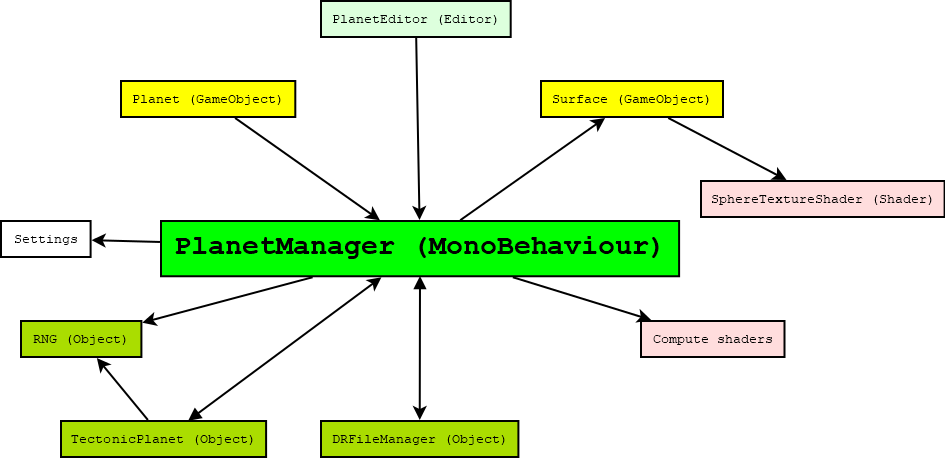
\includegraphics[width=15cm]{project-structure.png}
\caption{Simplified project structure}
\label{fig:project-structure}
\end{figure}
\subsection{TectonicPlanet object}
\asd{TectonicPlanet} is the most important data object in the project. It contains all relevant information about the simulated planet such as vertex positions, triangles, tectonic plate data, certain simulation statistics, vector noise, overlap relations and compute shader buffers. There are two main data layers, called \asd{Crust} and \asd{Data}. \asd{Crust} keeps all the tectonic model information and the simulation runs in this layer.  Because the data is interpreted as separated by plate, the layer mesh topology is broken along the plate borders. \asd{Data} layer provides compact surface data, i.~e. a~closed sphere surface mesh terrain (see Figure \ref{fig:model-layers}). Computed oceanic ridges information is only present in the \asd{Data} layer as it is not needed for plate interactions, only for resampling.
\begin{figure}[ht]
\centering
\begin{subfigure}{7cm}
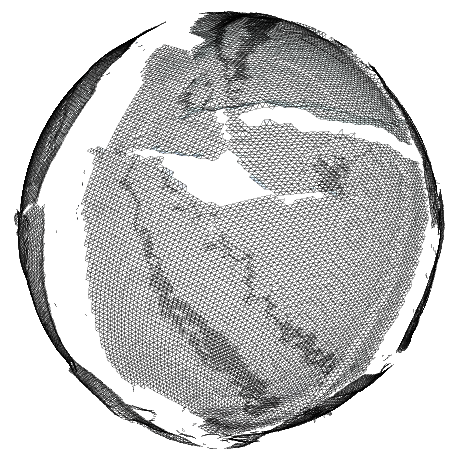
\includegraphics[height=7cm]{layer-crust.png}
\caption{crust}
\label{fig:layer-crust}
\end{subfigure}
\hspace*{1cm}
\begin{subfigure}{7cm}
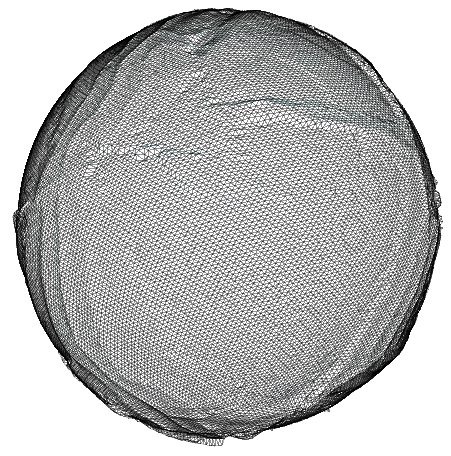
\includegraphics[height=7cm]{layer-data.png}
\caption{data}
\label{fig:layer-data}
\end{subfigure}\\
\begin{subfigure}{7cm}
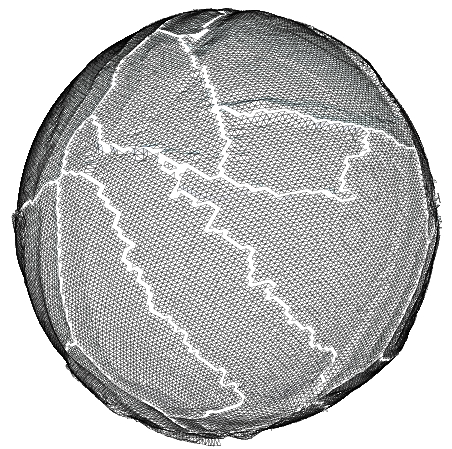
\includegraphics[height=7cm]{layer-resampled.png}
\caption{resampled crust}
\label{fig:layer-resampled}
\end{subfigure}
\caption{Model layers}
\label{fig:model-layers}
\end{figure}

Because Unity limits the number of vertices in a single mesh to the maximum UInt16 value 65,535 by default, another \asd{Render} layer is needed for rendering. It is essentially the same layer as \asd{Data}, but the information is interpolated onto a mesh with sufficiently low number of vertices.\footnote{There is a technique to render more detailed objects by splitting large meshes into chunks \cite{chunks}. In my opinion, however, this technique would add unnecessary complexity to the rendering process} The obvious problem with rendering can be seen in Figure \ref{fig:render-500k}.
\begin{figure}[ht]
\centering
\begin{subfigure}{7cm}
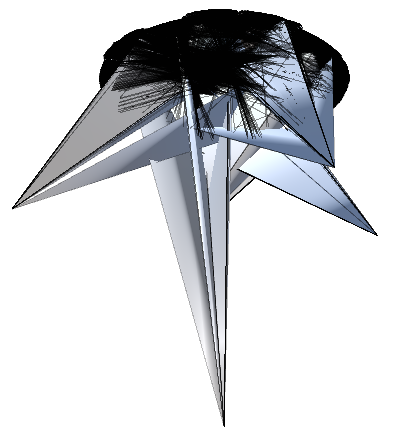
\includegraphics[height=7cm]{layer-toolarge.png}
\caption{data layer problem}
\label{fig:layer-toolarge}
\end{subfigure}
\hspace*{1cm}
\begin{subfigure}{7cm}
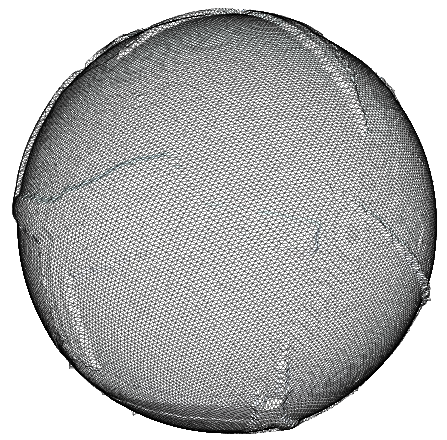
\includegraphics[height=7cm]{layer-render.png}
\caption{render layer correction at 60k vertices}
\label{fig:layer-render}
\end{subfigure}
\caption{Rendering of 500k vertices mesh}
\label{fig:render-500k}
\end{figure}
\subsubsection{Stored information}
Members of a~\asd{Planet} instance can be divided into three groups. First is the general information, including planet radius, reference to the \asd{PlanetManager} random number generator (as \asd{TectonicPlanet} heavily relies on it), vector noise data and the simulation statistics (the number of total tectonic steps performed and the number of tectonic steps performed since last resampling). The second group are the buffers needed for the compute shaders. These buffers store the planet state information in a~format suitable for GPU computing. The third group is the layer data (separately \asd{Crust}, \asd{Data} and \asd{Render}). It contains information about the vertex number and positions, the triangle number and geometry, vertex neighbours, triangle neighbours, triangles belonging to vertices, surface point data, tectonic plates and their overlap relations and the bounding volume hiearchy. Vertex positions are stored as a~list of \asd{Vector3} values, triangles are a~list of objects. Other members reference these by indexing. All members present in layers are stored separately. Description of individual layer data members follow.
\begin{itemize}[\label={}]
\item[\textbf{Vertex positions}] A~list of \asd{Vector3} type values representing positions of the samples on the unit sphere surface. These values do not change and tectonic drifts are represented by the plate quaternion transforms acting on vertex positions when needed. \asd{Crust} and \asd{Data} layer members are actually identical copies of the same information. Vertex indices point into this list.
\item[\textbf{Triangles}] A~list of \asd{DRTriangle} objects representing geometrical triangle data. Every instance has information about the vertex indices that comprise the triangle, its circumcircle, circumradius, centroid position, list of indicies of triangles sharing an edge and a~reference to the vertex position list. Again, the plate transforms are applied when needed. Triangle indices point into this list.
\item[\textbf{Vertex neighbours}] Nested \asd{int} list of indices of neighbouring vertices for each vertex (i.~e. by a~triangle edge). Index in the outer list corresponds to the index of a~vertex position.
\item[\textbf{Triangles of vertices}] Nested \asd{int} list of indices of triangles a~vertex is a~part of. vertices for each vertex (i.~e. by a~triangle edge). Index in the outer list corresponds to the index of a~vertex position.
\item[\textbf{Tectonic plates}] A~list of \asd{Plate} objects. Each instance has information about the vertices, triangles and border triangles belonging to the plate, its rotation axis, angular speed, transform, centroid position and plate-specific bounding volume hiearchy data. Plate indices point into this list.
\item[\textbf{Overlap relations}] A~two-index array antisymmetrical matrix representing the relation.
\item[\textbf{Surface point data}] A list of \asd{PointData} objects that store tectonic information: elevation, thickness, orogeny type, age and the plate index the vertex belongs to. The index in this list corresponds to the index of a~vertex position.
\item[\textbf{Bounding volume hiearchy}] Information for faster look-ups and collision tests. See subsection \ref{subsec:bvh}.
\end{itemize}

Initial data for a~new simulation are loaded from two template datafiles (their structure is described in Appendix \ref{sec:template-datafile-structure}) by the \asd{LoadDefaultTopology} method. A~template file contains the topology of a~Delaunay triangulation. One is used in the \asd{Data} layer and one in the \asd{Render} layer. No \asd{Crust} layer information is available until the simulation initializes the tectonic algorithm after some default topology is loaded.  There are several template files available with varying number of samples, but the \asd{Render} layer is limited by the maximum number of 60,000 samples.
\subsection{Bounding volume hiearchy}
\label{subsec:bvh}
During the simulation, the model performs searches in large sets of triangles many times, often for each element of another large set of vertices or triangles. Brute-force approach has the complexity of $\mathcal{O}(n^2)$. On the scale of around 100,000 elements, this adds up to $10^{10}$ iterations. Together with the fact that each iteration is not trivial to evaluate, this method is impractical. Driftworld uses bounding volume hiearches (BVH) to build a~binary search tree, reducing the total complexity to $n\log n$ \cite{sulaiman}\cite{bvharticle}.

Because the interaction space is the surface of a~unit sphere (i.~e. a~two-dimensional manifold), we choose the circumcircle as the bounding volume of a~triangle and the hiearchy is constructed from bottom up by merging circles. In \asd{Crust} layer each plate has its own BVH, \asd{Data} layer has one for the whole surface.
\subsubsection{Morton code}
Morton code is a technique which Driftworld uses to represent circle centers in an ordered manner \cite{morton}. Each circle can be assigned an \asd{UInt32} type value (synonymous to \asd{uint}) giving both coordinates inside a~grid on the sphere surface. The two spherical coordinates $\phi\in[0,2\pi)$ and $\theta\in[0,\pi]$ are normalized to intervals $\phi_1\in[0,1)$ and $\theta_1\in[0,1)$ and scaled to two \asd{UInt16} values:
$$\mbox{\asd{UInt16} }u_\phi=\lfloor 65535\phi_1\rfloor$$
$$\mbox{\asd{UInt16} }u_\theta=\lfloor 65535\theta_1\rfloor$$
The individual bits of the binary representations of $u_\phi$ and $u_\theta$ are then interlaced in a single \asd{UInt32} value $u_{\phi\theta}$ so that the least significant bit of $u_\phi$ is the least significant bit of $u_{\phi\theta}$.

\paragraph{Example} A circle has a center $\mathbf{c}(\phi,\theta)$ at (3.1,0.5). The normalized values are $\phi_1=0.493,\theta_1=0.159$. The binary representations of $u_\phi, u_\theta$ and $u_{\phi\theta}$ are:
$$u_\phi=\mbox{0111 1110 0011 010\underline{0}}$$
$$u_\theta=\mbox{0010 1000 1011 0100}$$
$$u_{\phi\theta}=\mbox{0001 1101 1101 0100 1000 1111 0011 000\underline{0}}$$
\subsubsection{Constructing BVH}
The hiearches are constructed for sets of triangles. Each triangle must provide the positions of its vertices. From this information, the circumcenters and the circumradii are calculated, which are the elementary bounding volumes. These elementary volumes become the leaves of the hiearchy tree. The construction loop begins with the merging of some suitable couples of circles, creating parent node larger circles. These new circles together with the unmerged circles become the new set of circles for the new loop iteration. The loop repeats until a single root circle is created (see Figure \ref{fig:bvh-construction}).
\begin{figure}[ht]
\centering
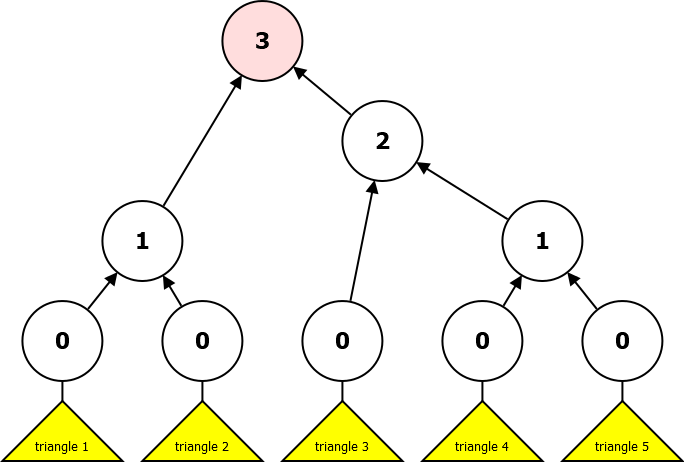
\includegraphics[width=14cm]{bvh-construction.png}
\caption{Example of a BVH construction over 5 triangles in 3 iterations}
\label{fig:bvh-construction}
\end{figure}

Merging circles randomly creates unreasonably large bounding volumes on lower levels of a BVH. It is therefore useful to identify close circles to avoid wasting space. Determining nearby clusters by brute-force has a complexity of $\mathcal{O}(n^2)$ at least, not considering cases where the nearest neighbour relation is not mutual. Because of that, Driftworld utilizes a~parallel search for suitable circle couples to be merged \cite{meister}. In each iteration, the set of circles is bucket-sorted by their Morton codes into an array. Then for each element a~candidate is selected within a range of $r_M=20$ elements (clamped to the array borders) that is the nearest and its index is flagged. If two elements are the nearest candidates of each other, their respective bounding volumes are merged for the next iteration.
\subsubsection{Searching the BVH}
Because of memory restrictions of the L1 cache of the GPU (trees are searched by compute shaders), Driftworld implements a~DFS algorithm for determining collisions or finding vertices inside triangles. The tree is searched using left-child-first rule, traversing left children first and rejecting all nodes (and their children) whose bounding volumes do not meet the collision parameters. The search stops when a colliding triangle is found or when the whole hiearchy is searched with no hit. An example of a~traversal is seen in Figure \ref{fig:dfs-traversal}. Dashed circles do not meet the collision parameters, green triangles are hits. Only the first triangle hit is considered when traversing.

The algorithm uses a~stack with the maximum size of $d_s=40$, which remembers the current path of the tree traversal.
\begin{figure}[ht]
\centering
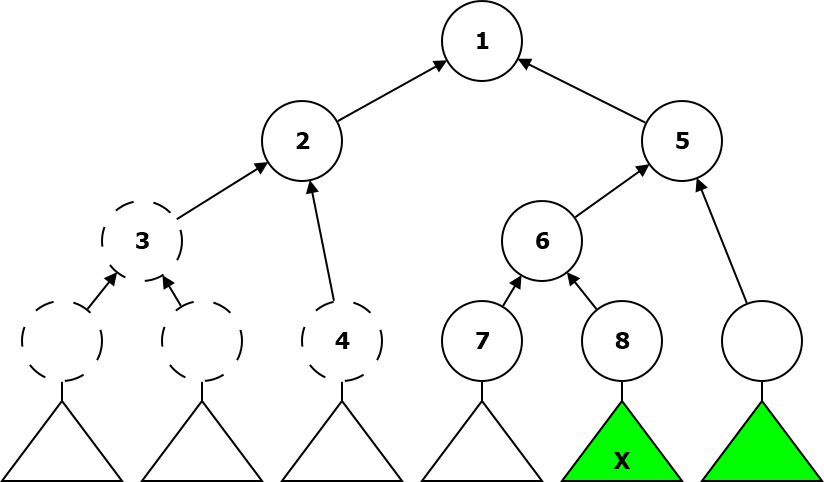
\includegraphics[width=14cm]{dfs-search-A.png}
\caption{Example of a tree traversal order}
\label{fig:dfs-traversal}
\end{figure}
\subsection{GPU Computing}
The number of processing-intensive tasks that are performed each step requires a~faster implementation using compute shaders. \asd{TectonicPlanet} stores a~dictionary of \asd{ComputeBuffer} instances. The buffers are updated only when relevant data is changed, using a~\asd{bool} dictionary for flagging. All buffers are interpreted as one-index array of either primitive types or specially designed structs understandable by the shaders. Two-dimensional arrays representing a~list of lists are accompanied by so-called sps buffer arrays with pivot points dividing individual lists. All buffers remain active in the memory unless rewritten by loading another simulation.
\begin{itemize}[\label={}]
\item[\textbf{BVH nearest neighbour shader}] Used for determining the nearest bounding volume candidates for constructing BVH. Run once per construction iteration.
\item[\textbf{Vertex data interpolation shader}]  Used for translating data between planet data layers. Interpolates point data to mesh of the correspondent layer.
\item[\textbf{Plate interactions shader}] Used for the majority of look-ups during tectonic steps.  It is the most complex shader with numerous different kernels, responsible for testing border collisions with plates, subduction uplift, continental erosion, oceanic damping, sediment accretion, slab pull contributions, contacts between continental triangles and continental collision uplift.
\item[\textbf{Overlay texture shader}] Computes pixel colors for 4096x4096 textures used in displaying data on the surface mesh.
\item[\textbf{Fractal terrain shader}] Computes changes in elevation in one fractal terrain generation iteration. This is not a~part of the Driftworld tectonic simulation.
\end{itemize}

\subsection{Precision issues}
Driftworld tools use almost exclusively \asd{float} precision because \asd{Vector3} components are of \asd{float} type and the shaders utilize FP32 cores. For the most part, 32-bit precision does not pose a problem, but sometimes certain operations suffer from rounding errors. Most notably, \asd{acos} function is used to compute distances from dot products. In some cases, a~dot product result of assumed unit vectors is greater than 1. This is obviously outside the domain of \asd{acos}, so the values are clamped to 1 manually. During BVH look-ups, the BV collisions are tested by comparing distances from the BV centers with their radii. The value of any BV radius is overestimated by 1~\% during tree traversals. This obviously decreases the efficiency of the algorithm, but also decreases the chance of a~correct BVH branch being rejected. When testing whether a point is inside a triangle, there is a tolerance of $10^{-4}$ for the results of dot products with the normals of the edge planes.

The template mesh files provide the sample position coordinates in \asd{double} precision. These need to be converted to \asd{float} when reading.
\subsection{Rendering}
\label{subsec:rendering}
Unity was chosen for this project in large part because of the ease with which data can be visualized. The \asd{Surface} GameObject is a dedicated Object in the scene used for rendering the planet surface. It can render any of the three data layers with the exception of the template mesh files with over 60,000 samples (that should be used exclusively in the \asd{Crust}/\asd{Data} layers). During rendering, the mesh takes elevation into account, despite it being separately stored in the crust point objects. The rendering has three parts: basic mesh, elevation and overlay (see subsection \ref{subsec:overlays}). The basic mesh consists of the crust vertices, which always have a~length of the planet radius $R$, and the triangles. In case of \asd{Crust} and \asd{Data} layers all triangles of the surface mesh are fed to the \asd{MeshFilter} component. The \asd{Crust} layer only considers triangles that are entirely a part of a tectonic plate. This is because triangles between plates have distorted geometry due to the plate transforms. The elevation part is used for adjusting the length of mesh vertices to visualize surface details. Any unit vertex $\mathbf{u}_i$ on the surface has an accompanying elevation value $z_i$. The actual vertex that is fed to the \asd{MeshFilter} is:
$$\mathbf{u}_i'=(R+h_ez_i)\mathbf{u}_i$$
$h_e=50$ is the elevation scale factor used for stressing the surface features. The vertices are fed through an array of \asd{Vector3} values and the triangles are a~one-dimensional sequential array of triples of indices within the vertex array.

Figure \ref{fig:render-layers} shows examples of renders of the same simulation state in different layers. Faults in the plate topology are clearly seen in Figure \ref{fig:render-crust}. Figure \ref{fig:render-data} shows full \asd{Data} layer mesh with prominent surface features. The relative decrease in the \asd{Render} layer mesh resolution is shown in Figure \ref{fig:render-normal}, although since the overlays are computed at the \asd{Data layer}, some details are preserved in the texture. Setting the elevation scale to 1 (true relative scale) reveals how the terrain has very little influence on the apparent surface from distance (Figure \ref{fig:render-escale1}).

User can choose to clamp the render to the ocean level, hiding all surface details below the ocean level. The ocean would appear as somewhat spherical portion of the planet.

\begin{figure}[ht]
\centering
\begin{subfigure}{7cm}
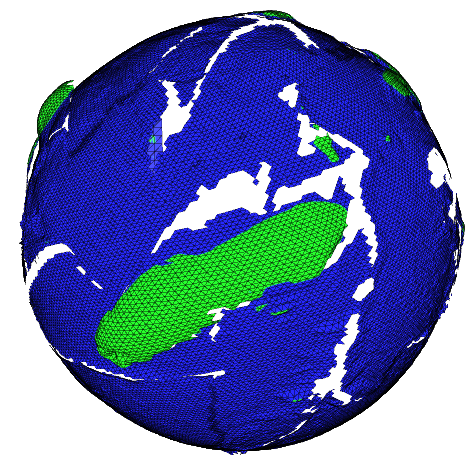
\includegraphics[height=7cm]{render-crust.png}
\caption{crust layer at 60,000 samples}
\label{fig:render-crust}
\end{subfigure}
\hspace*{1cm}
\begin{subfigure}{7cm}
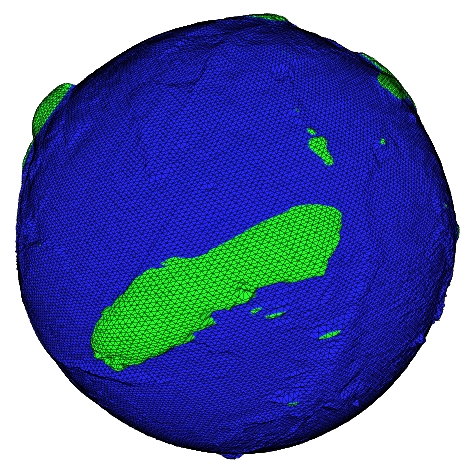
\includegraphics[height=7cm]{render-data.png}
\caption{data layer at 60,000 samples}
\label{fig:render-data}
\end{subfigure}\\
\begin{subfigure}{7cm}
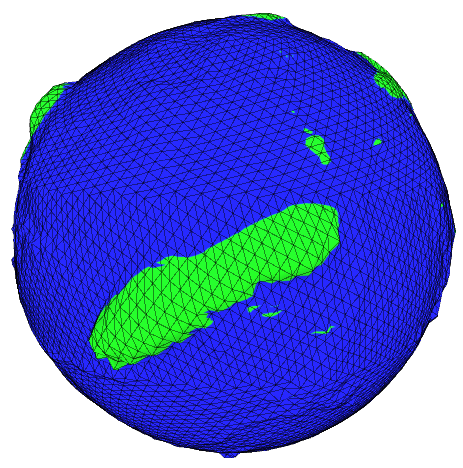
\includegraphics[height=7cm]{render-normal.png}
\caption{render layer at 10,000 samples}
\label{fig:render-normal}
\end{subfigure}
\hspace*{1cm}
\begin{subfigure}{7cm}
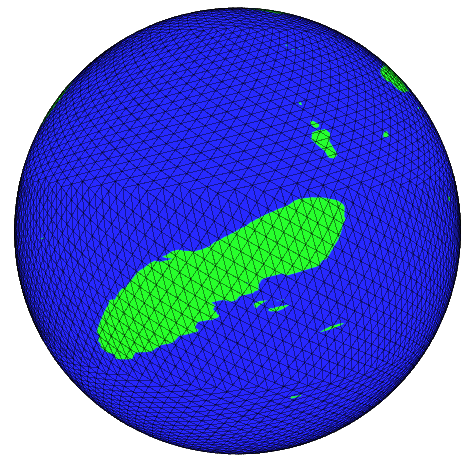
\includegraphics[height=7cm]{render-escale1.png}
\caption{render layer with elevation scale 1}
\label{fig:render-escale1}
\end{subfigure}
\caption{Renders with the basic terrain overlay}
\label{fig:render-layers}
\end{figure}
\subsection{Overlays}
\label{subsec:overlays}
Overlay is a \asd{Texture2D} image assigned to the \asd{Renderer} component \asd{\_MainTex} property of the \asd{Surface} GameObject. Any overlay is computed by the Overlay texture compute shader on-the-fly before assignment. There is a~number of different overlays implemented for checking the state of the simulation. The user can select between them independently of the layer chosen. The render does not require an overlay, leaving the object with the basic white albedo. Figure \ref{fig:overlay-render} shows examples of overlay renders with the same simulation state as Figure \ref{fig:render-layers}. Texture pixels use barycentric interpolation.
\begin{figure}[ht]
\centering
\begin{subfigure}{4cm}
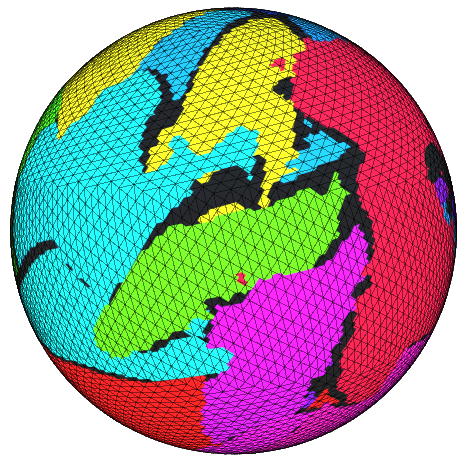
\includegraphics[height=4cm]{overlay-crustplates.png}
\caption{crust plates}
\label{fig:overlay-crustplates}
\end{subfigure}
\hspace*{1cm}
\begin{subfigure}{4cm}
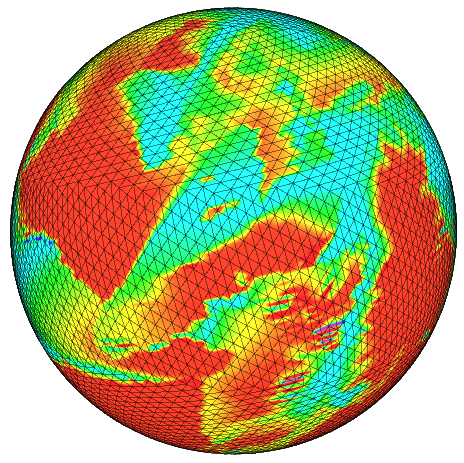
\includegraphics[height=4cm]{overlay-crustage.png}
\caption{crust age}
\label{fig:overlay-crustage}
\end{subfigure}
\hspace*{1cm}
\begin{subfigure}{4cm}
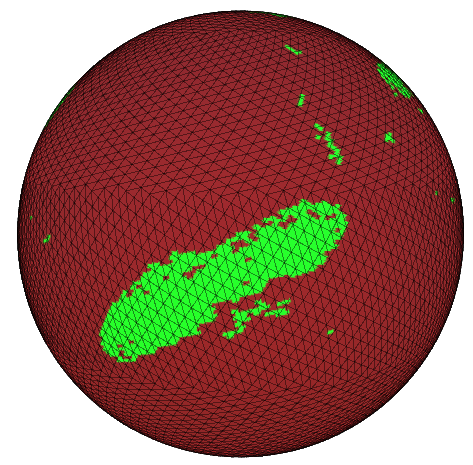
\includegraphics[height=4cm]{overlay-orogeny.png}
\caption{orogeny}
\label{fig:overlay-orogeny}
\end{subfigure}\\
\begin{subfigure}{4cm}
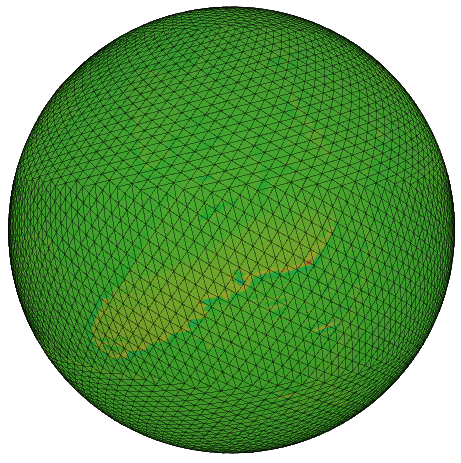
\includegraphics[height=4cm]{overlay-elevationlaplacian.png}
\caption{elevation Laplacian}
\label{fig:overlay-elevationlaplacian}
\end{subfigure}
\hspace*{1cm}
\begin{subfigure}{4cm}
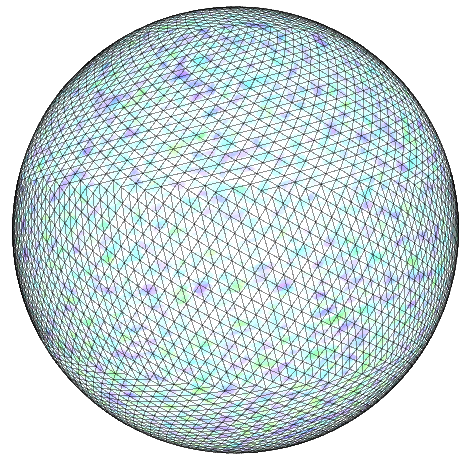
\includegraphics[height=4cm]{overlay-vectornoise.png}
\caption{vector noise}
\label{fig:overlay-vectornoise}
\end{subfigure}
\hspace*{1cm}
\begin{subfigure}{4cm}
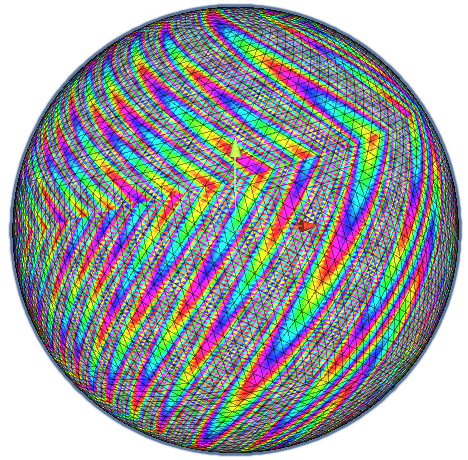
\includegraphics[height=4cm]{overlay-debugdatatriangles.png}
\caption{debug triangles}
\label{fig:overlay-debugtriangles}
\end{subfigure}\\
\caption{Overlay examples}
\label{fig:overlay-render}
\end{figure}
\begin{itemize}[\label={}]
\item[\textbf{Basic terrain}] This is the primary overlay. It is a simplified texture, differentiating between crust points below and above the ocean level. Points below the ocean level (zero elevation) have blue pixels, green otherwise. There is an error state overlay, such as when missing data for computing a~texture. It is a~solid bright red overlay.
\item[\textbf{Crust plates}] Domains of individual tectonic plates are shown. They are distinguished by the color hue.
\item[\textbf{Crust age}] Colors represent relative crust age. Red hue is for the oldest crust, blue for the newest near the oceanic ridges. Hue increases on a~standard color wheel.
\item[\textbf{Orogeny}] Three colors distinguish between different orogenies. Dark red is of None type, green is for Andean, blue for Himalayan.
\item[\textbf{Elevation Laplacian}] Used for detecting large slopes in elevation. Green is for relatively flat mesh, redder are for peaks.
\item[\textbf{Vector noise}] The representation of the simulation vector noise. Hue determines relative direction, saturation the intensity of the noise.
\item[\textbf{Debug data triangles}] Individual triangles in the \asd{Data} layer are painted in different hues. Mesh triangle ordering patterns are visible.
\item[\textbf{Debug crust triangles}] The same as for data triangles, although in the \asd{Crust} layer. Points between plates are painted black like the door.
\end{itemize}
\subsection{No amplification}
At the present state the amplification methods discussed by Cortial et al. are not implemented. Subsequent processing is possible for the saved simulations. This, however, requires interpolating the data onto a finer mesh. A~first-person agent would percieve the surface as nearly flat. The simplest method for enhancing the simulated surface could be a multi-frequency Perlin noise. Lack of an~amplified terrain should not seriously alter simulations such as hydrosphere.
\subsection{Random number generator}
Random numbers are used for initializing plates, creating vector noise, rifting events, safeguarding precision error cases and creating a~reference random fractal terrain. Standard linear congruential generators are insufficient for any advanced simulations, so Driftworld uses an implementation of a~Mersenne Twister. The implementation code is adapted from a~website example by PROWAREtech \cite{prowaretech}.

There is a single instance of the generator to assure consistent results. The state can be reset by providing a~seed parameter. The state of the generator is saved along the data when saving the simulation state to a~file.
\subsection{Use}
User has relatively large control over different aspects of the simulation. All model parameters can be changed in the inspector even between steps. The inspector controls show a~degree of accessibility logic, such as not being able to perform tectonic steps without initialized plates etc.

The inspector has several sections. First are the basic settings. Template data filenames for the \asd{Data} and \asd{Render} layers are the files that are read when loading a~fresh new simulation. Save filename is used to store ongoing simulation. The texture save filename is for saving any overlays as a~PNG image. The random number generator seed is for initializing the Mersenne Twister either before starting a~new simulation or between tectonic steps. The number of tectonic steps are performed in sequence per one activation. Lastly, the elevation scale factor was discussed in subsection \ref{subsec:rendering}.

\asd{PlanetManager} keeps an instance of two serializable sets of settings. The main settings collection  keeps all model parameters and other too, such as the Morton array look-up radius $r_M$. The shader settings are used to assign shader files. These are referenced whenever a kernel dispatch is to be called.

The overview section in the inspector shows some basic information about the simulation state. If a~loaded planet simulation is present, the overview shows the number of vertices and triangles both in \asd{Data} and \asd{Render} layer. Current rendering mode is displayed, although the user can check it in the render options. Current number of tectonic plates is important for fine-tuning the rifting frequency. Simulation statistics show the total number of tectonic steps taken and the number of tectonic steps taken without resampling.

A~fresh new simulation is loaded by the \asd{Load new planet} button. Correct filenames must be provided in the settings or the default topology load will fail. When an instance of \asd{TectonicPlanet} is active, it is possible to save the state by the \asd{Save planet to file} button. \asd{Load planet from file} overwrites any current simulation by loading a~saved simulation state from a~file. Correct filename must be provided. Note that rewriting the current simulation by any other, as well as changing a~script code (and forcing Unity to recompile) voids the current compute buffers. These must be cleared before changing the simulation in this way.

Render options are a~set of tools to look at different aspects of the simulation. User can choose an overlay or a~layer to render. Several switches control if the data should be automatically interpolated onto higher levels when needed (\asd{Crust} $\rightarrow$ \asd{Data} $\rightarrow$ \asd{Render}), if the render is clamped to the ocean level or whether the overlays should be painted over the rendered object or not. \asd{Wash texture} removes any overlay currently displayed and \asd{Render surface} renders the object with any new settings without performing a~tectonic step.

Tectonic tools are the main controls of the simulation. \asd{Initialize tectonic plates} creates a new random tectonic configuration (it a actually starts a~new simulation on a~loaded mesh). This allows for the tectonic steps to be performed. Any part of the tectonic simulation can be switched for fine-tuning or adjusting the simulation. \asd{Resample crust} manually forces resampling of \asd{Crust} layer data. Tectonic step is the manual activation tool to perform a~sequence of tectonic steps set above (1 is recommended for purposes other than fine-tuning). Calling for plates initialization requires clearing the buffers.

Data manipulation has several tools to help adjust the simulation. Clearing the buffers is the most important if the user wants to load another simulation or make changes to the script code. Smoothing elevation flattens the terrain by neighbour elevation averaging. It uses a~\textit{neighbour smooth} parameter $z_s=0.1$ , which represents the weight of the neighbour elevation when averaging. Laplacian smooth elevation performs a~similar action, however the weights are differences in elevation scaled to the maximum elevation range. RNG initialization resets the random number generator to the state denoted by a~set seed. Calculating thickness is a~placeholder action that recalculates the default thickness (this crust point information is not implemented in a~contextual manner). Forcing a~plate rift creates two new randomly divided plates from the largest plate in the \asd{Crust} layer. User can export an~overlay texture at any time, provided there is one rendered.

There is the possibility of creating a~standard fractal terrain. This does not simulate orogeny, crust age or other aspects of the tectonic simulation. It takes place entirely within the \asd{Data} layer. There are two main parameters that drive the fractal terrain generation: fractal terrain elevation step $z_f=0.003\mbox{ u}$ and fractal terrain iterations $n_f=10,000$. It runs in a~loop of $n_f$ iterations.  Each iteration chooses a~random plane passing the origin and changes elevation of every \asd{Data} point by $z_f$ -- increases on one side of the plane, decreases on the other. Data from fractal terrain generation can be used to a~degree, but the user must keep in mind that only elevation values are created. For quicker computation, fractal terrain generation uses a~dedicated compute shader and the random normal vectors of the planes are provided beforehand to the dispatched kernel. The elevations are computed for each point independently (one thread -- one vertex). Also note that the parameters $z_f$ and $n_f$ depend on each other.

Diagnostic tools are used to check the sanity of the topology and elevation. \asd{BVH Diagnostics} checks the bounding volume hiearchies for both \asd{Crust} and \asd{Data} layers, showing basic information about the look-up trees. The most relevant information is the tree depth, because a healthy tree should have a~depth of around $\log_2n$, where $n$ is the number of triangles in the hiearchy. \asd{Mesh and elevation value diagnostics} checks the sanity of the mesh. Vertex magnitude is evaluated (should be 1 within tolerance of 0.0001) and the elevation values must not have a \asd{NaN} or some infinity value. All layers are checked.

There is a~group of four work-in-progress tools that are blank. Their code can be adjusted for debugging or trying new things. They have a~wide access to all simulation data.
\begin{table}[h]
\centering
\begin{tabular}{ccc}
\textbf{Symbol}&\textbf{Description}&\textbf{Value}\\
\hline
$r_M$&Morton array look-up radius&20\\
$d_s$&Maximum stack size for DFS search&40\\
-&Bounding volume radius tolerance&1 \%\\
-&Triangle interior test tolerance&$10^{-4}$\\
$h_e$&Elevation scale factor&50\\
$z_s$&Neighbour smooth parameter&0.1\\
$z_f$&Fractal terrain elevation step&0.003\mbox{ u}\\
$n_f$&Fractal terrain iterations&10,000\\
\end{tabular}
\caption{Implementation parameters summary}
\label{tab:implementation-parameters-summary}
\end{table}